\documentclass[12pt,letterpaper]{article}
\usepackage[utf8]{inputenc}
\usepackage[spanish]{babel}
\usepackage{graphicx}
\usepackage[left=2cm,right=2cm,top=2cm,bottom=2cm]{geometry}
\usepackage{graphicx} % figuras
% \usepackage{subfigure} % subfiguras
\usepackage{float} % para usar [H]
\usepackage{amsmath}
%\usepackage{txfonts}
\usepackage{stackrel} 
\usepackage{multirow}
\usepackage{enumerate} % enumerados
\renewcommand{\labelitemi}{$-$}
\renewcommand{\labelitemii}{$\cdot$}
% \author{}
% \title{Caratula}
\begin{document}

% Fancy Header and Footer
% \usepackage{fancyhdr}
% \pagestyle{fancy}
% \cfoot{}
% \rfoot{\thepage}
%

% \usepackage[hidelinks]{hyperref} % CREA HYPERVINCULOS EN INDICE

% \author{}
\title{Caratula}

\begin{titlepage}
\begin{center}
\large{UNIVERSIDAD PRIVADA DE TACNA}\\
\vspace*{-0.025in}
\begin{figure}[htb]
\begin{center}

\includegraphics[width=8cm]{./Imagenes/logo}
\end{center}
\end{figure}
\vspace*{0.15in}
INGENIERIA DE SISTEMAS  \\

\vspace*{0.5in}
\begin{large}
TITULO:\\
\end{large}

\vspace*{0.1in}
\begin{Large}
\textbf{TRABAJO FINAL DE UNIDAD I} \\
\end{Large}

\vspace*{0.3in}
\begin{Large}
\textbf{CURSO:} \\
\end{Large}

\vspace*{0.1in}
\begin{large}
BASE DE DATOS II\\
\end{large}

\vspace*{0.3in}
\begin{Large}
\textbf{DOCENTE(ING):} \\
\end{Large}

\vspace*{0.1in}
\begin{large}
 Patrick Cuadros Quiroga\\
\end{large}

\vspace*{0.2in}
\vspace*{0.1in}
\begin{large}
Integrantes: \\
\begin{flushleft}
Balaguer Valles Angela Lesslie	\hfill	(2016054494) \\
Huallpa Castro Leydi Katherine	\hfill	(2015053230) \\
Mamani Ayala  Brandon \hfill  (2015052715) \\
Pilco Quispe Mireya Flavia	\hfill  (2015053234) \\
Quispe Mamani Angelo        \hfill	(2015052826) \\
Vizcarra Llanque Jhordy        \hfill	(2015052719) \\
\end{flushleft}
\end{large}
\end{center}

\end{titlepage}


\tableofcontents % INDICE
\thispagestyle{empty} % INDICE SIN NUMERO
\newpage
\setcounter{page}{1} % REINICIAR CONTADOR DE PAGINAS DESPUES DEL INDICE

\section{PROBLEMA} 

\section{MARCO TEORICO} 
A través de los años los sistemas de administración de Bases de Datos han
evolucionado hacia Sistemas de Administración de Base de Datos Relacionales
(RDBMS). Una base de datos relacional es un modelo organizado de entidades
que posee características que tienen relaciones entre ellas. Una base de datos
relacional bien diseñada provee información de un negocio o un proceso y su uso
más común es para almacenar y recuperar información. Entre las mayores
ventajas de RDBMS están la forma en la que almacena y recupera información y
cómo mantiene la integridad de la misma. Las estructuras RDBMS son fáciles de
comprender y construir, pues son lógicamente representadas utilizando Diagramas
Entidad-Relación. Las bases de datos relacionales tienen las siguientes
características principales: 
\begin{itemize}
\item
• Estructuras. Son objetos que almacenan o acceden a los datos de la base
de datos (Tablas, vistas e índices). 
\item
• Tabla. Es un objeto que almacena datos en forma de filas y columnas. Cada
tabla tiene una o más columnas y filas. Las columnas guardan una parte de
la información sobre cada elemento que queremos guardar en la tabla, cada
fila de la tabla conforma un registro. Los datos de una tabla contienen valores
atómicos, es decir que contiene elementos indivisibles.
\item
• Integridad. La integridad de la base de datos se refiere a la validez y la
consistencia de los datos.
\item
• Facilidad de uso. Los usuarios tendrán fácil acceso a los datos. Las
complejidades internas son ajenas al usuario, gracias al sistema de
administración de la base.
\item
• Redundancia controlada. Los datos serán almacenados una sola vez
excepto cuando existan razones técnicas o económicas que aconsejen el
almacenamiento redundante.
\item
• Seguridad de acceso. Se evitará el acceso no autorizado de datos. Los
mismos podrán estar sujetos a diferentes restricciones de acceso para
distintos usuarios.
\item
• Operaciones. Son acciones usadas para definir las Estructuras o manipular
los datos de las mismas (SELECT, CREATE)
\item
• Reglas de integridad. Gobiernan los tipos de acciones permitidas en los
datos y la estructura de la Base de Datos (BD). Protegen los datos y
estructuras de la BD. (Llaves primarias y foráneas).
\item
• Identificador único. No pueden existir dos tablas con el mismo nombre, así
como no pueden existir dos columnas con el mismo nombre en una misma
tabla y los valores almacenados en una columna deben ser del mismo tipo
de dato.
\item
• Clave única. Cada tabla puede tener uno o más campos cuyos valores
identifican de forma única cada registro de dicha tabla, es decir, no pueden
existir dos o más registros diferentes cuyos valores en dichos campos sean
idénticos. Este conjunto de campos se llama clave única. 
\item
• Clave primaria. Una clave primaria es una clave única elegida entre todas
las candidatas que define unívocamente a todos los demás atributos de la
tabla, para especificar los datos que serán relacionados con las demás
tablas. La forma de hacer esto es por medio de claves foráneas. Sólo puede
existir una clave primaria por tabla y ningún campo de dicha clave puede
contener valores NULL.
\item
• Dominios. Un dominio describe un conjunto de posibles valores para cierto
atributo. Como un dominio restringe los valores del atributo, puede ser
considerado como una restricción. Matemáticamente, atribuir un dominio a un
atributo significa "todos los valores de este atributo deben de ser elementos
del conjunto especificado".
\item
• Normalización. Las bases de datos relacionales pasan por un proceso al
que se le conoce como normalización, el resultado de dicho proceso es un
esquema que permite que la base de datos sea usada de manera óptima.

    \item Una base de datos es un “almacén” que nos permite guardar grandes cantidades de información de forma organizada para que luego podamos encontrar y utilizar fácilmente.

Ademas se esta utilizando Visual studio que ha sido desarrollado con el objetivo de entregar a los usuarios de programación informática un paquete de utilidades simples y accesibles. Es por esto que Visual Studio puede ser usado y fácilmente comprendido por expertos como también por usuarios principiantes. Visual studio es además un lenguaje de programación guiado por eventos que permite mayor operatibilidad y mejores resultados.

La creación de interfaces gráficas para diferentes utilidades es una de las principales funciones del Visual Studio y es por esto que es altamente usado en espacios profesionales donde se requieren soportes gráficos para mayor organización de los contenidos y materiales. La programación gráfica se puede llevar a cabo directamente ya que el Visual studio no requerirá de los usuarios la escritura de los códigos de programación. Visual studio trabaja a partir de lenguajes RAD, en inglés Rapid Application Development, o desarrollo rápido de aplicaciones específicas para cada necesidad y función. Al mismo tiempo, el Visual studio, gracias a su simple lenguaje, es perfectamente adaptable a las plataformas de los sistemas Windows y es fácilmente transformable a otros lenguajes más complejos.

Microsoft ha desarrollado numerosas versiones para Visual studio. Una de las más antiguas data de 1992 y si bien presentaba el lenguaje en forma de texto, permitía ya disfrutar y acceder a algunos de los elementos más importantes del futuro Visual studio. Hoy en día, la versión 2015 es la más difundida a nivel mundial gracias a la combinación de elementos simples y de elementos perfeccionados.


\end{itemize}
\section{DESARROLLO} 
\subsection{ANALISIS (CASOS DE USO, SECUENCIAS, ACTIVIDADES)}
\subsubsection{CASOS DE USO}
\thinspace
\thinspace
\thinspace
\thinspace
\thinspace
\thinspace
\thinspace
\thinspace
\thinspace
\thinspace
\thinspace
\thinspace
\thinspace
\thinspace
\thinspace
\thinspace
\begin{center}
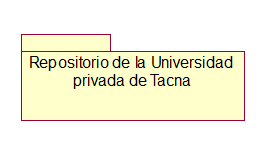
\includegraphics[width=8cm]{./Imagenes/CasoUso1}
\end{center}
\thinspace
\thinspace
\thinspace
\thinspace
\thinspace
\thinspace
\thinspace
\thinspace
\thinspace
\thinspace
\thinspace
\thinspace
\thinspace
\thinspace
\thinspace
\thinspace
\thinspace
\begin{center}
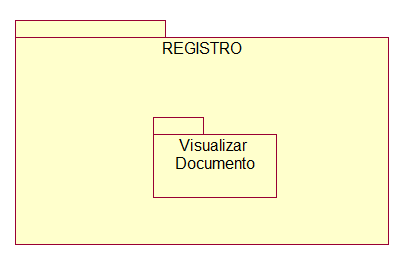
\includegraphics[width=8cm]{./Imagenes/CasoUso2}
\end{center}	
\thinspace
\thinspace
\thinspace
\thinspace
\thinspace
\thinspace
\thinspace
\thinspace
\thinspace
\thinspace
\thinspace
\thinspace
\thinspace
\thinspace
\thinspace
\thinspace
\thinspace
\thinspace
\thinspace
\thinspace
\thinspace
\thinspace
\thinspace
\thinspace
\thinspace
\thinspace
\begin{center}
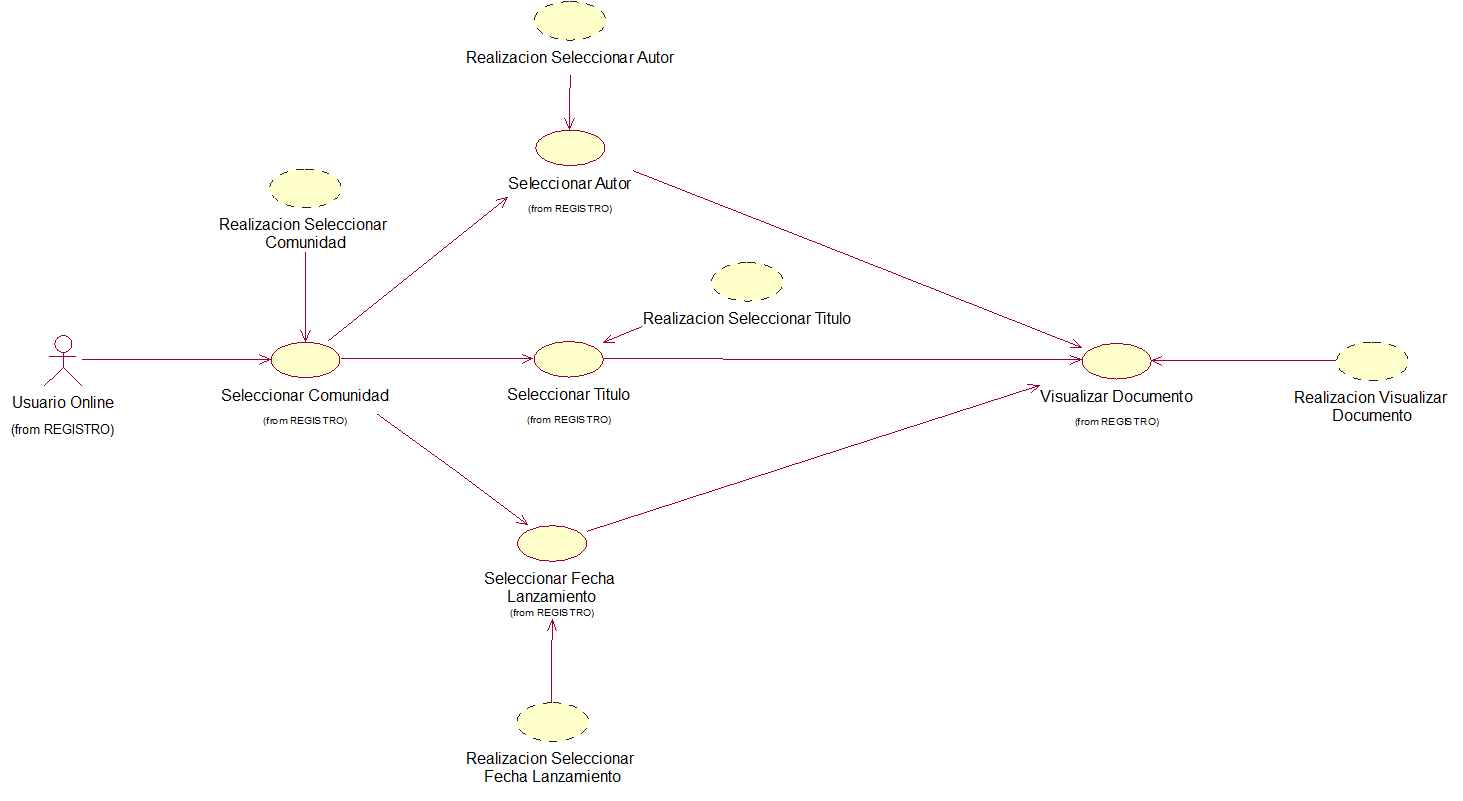
\includegraphics[width=18cm]{./Imagenes/CasoUso3}
\end{center}
\subsubsection{DIAGRAMA DE SECUENCIA}
\subsubsection{DIAGRAMA DE SECUENCIA}
\thinspace
\thinspace
\thinspace
Seleccionar Comunidad
\thinspace
\thinspace
\thinspace
\thinspace
\thinspace
\thinspace
\thinspace
\thinspace
\thinspace
\thinspace
\thinspace
\thinspace
\begin{center}
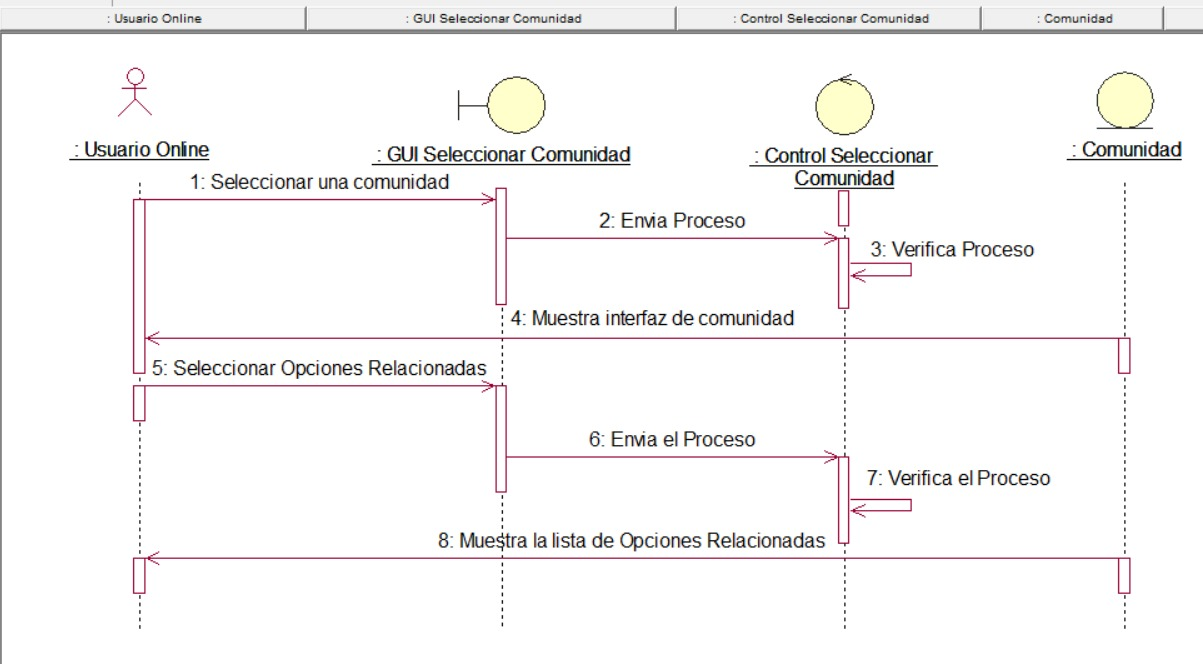
\includegraphics[width=14cm]{./Imagenes/Secuencia1}
\end{center}
\thinspace
\thinspace
\thinspace
\thinspace
\thinspace
\thinspace
\thinspace
\thinspace
\thinspace
\thinspace
\thinspace
\thinspace
\thinspace
\thinspace
Seleccionar Autor
\thinspace
\thinspace
\thinspace
\thinspace
\thinspace
\thinspace
\thinspace
\thinspace
\thinspace
\thinspace
\thinspace
\thinspace
\begin{center}
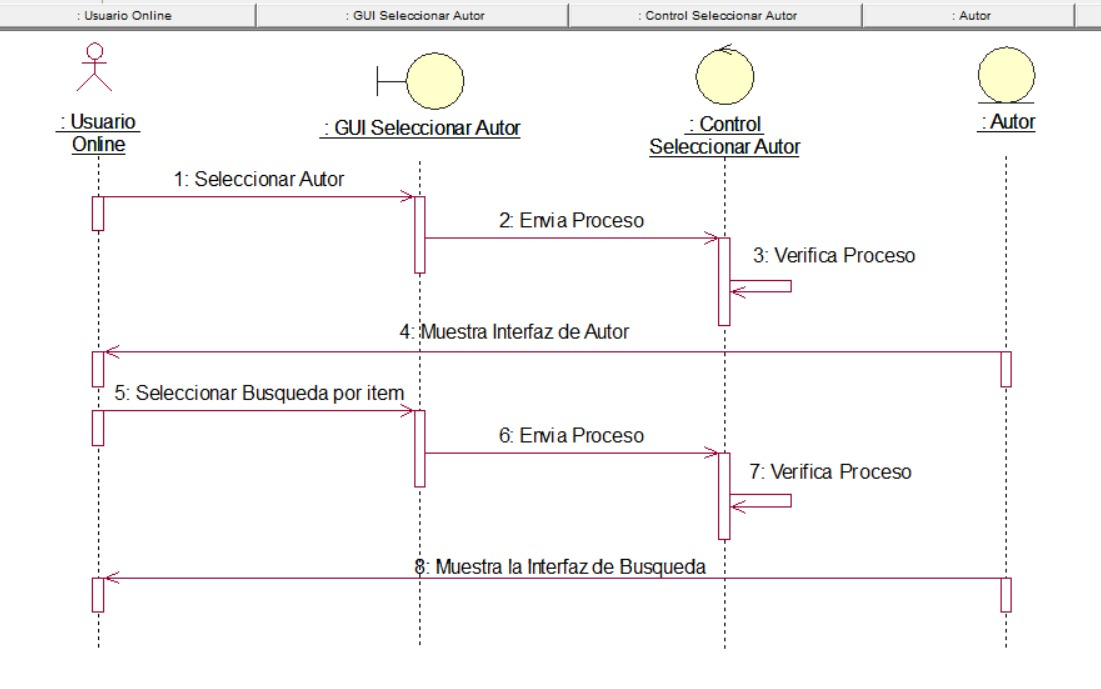
\includegraphics[width=14cm]{./Imagenes/Secuencia2}
\end{center}
\thinspace
\thinspace
\thinspace
\thinspace
\thinspace
\thinspace
\thinspace
\thinspace
\thinspace
\thinspace
\thinspace
\thinspace
\thinspace
\thinspace
Seleccionar Titulo
\thinspace
\thinspace
\thinspace
\thinspace
\thinspace
\thinspace
\thinspace
\thinspace
\thinspace
\thinspace
\thinspace
\thinspace
\begin{center}
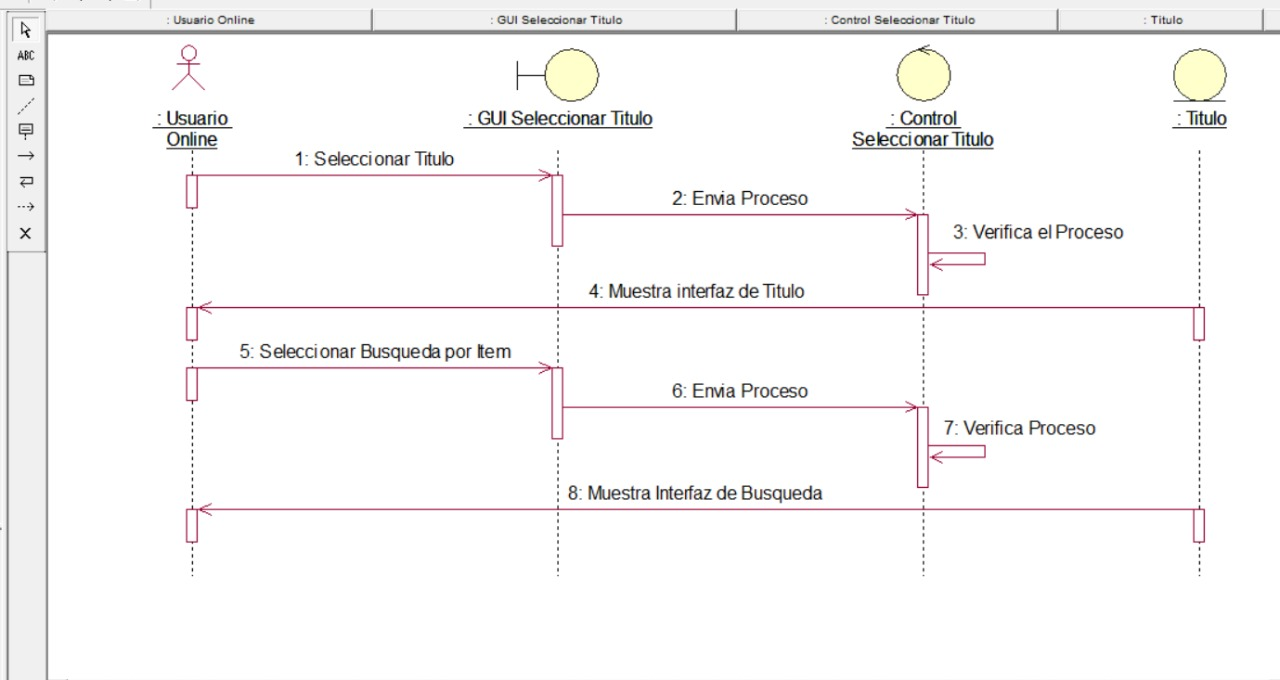
\includegraphics[width=14cm]{./Imagenes/Secuencia3}
\end{center}
\thinspace
\thinspace
\thinspace
\thinspace
\thinspace
\thinspace
\thinspace
\thinspace
\thinspace
\thinspace
\thinspace
\thinspace
\thinspace
\thinspace
Seleccionar Año
\thinspace
\thinspace
\thinspace
\thinspace
\thinspace
\thinspace
\thinspace
\thinspace
\thinspace
\thinspace
\thinspace
\thinspace
\begin{center}
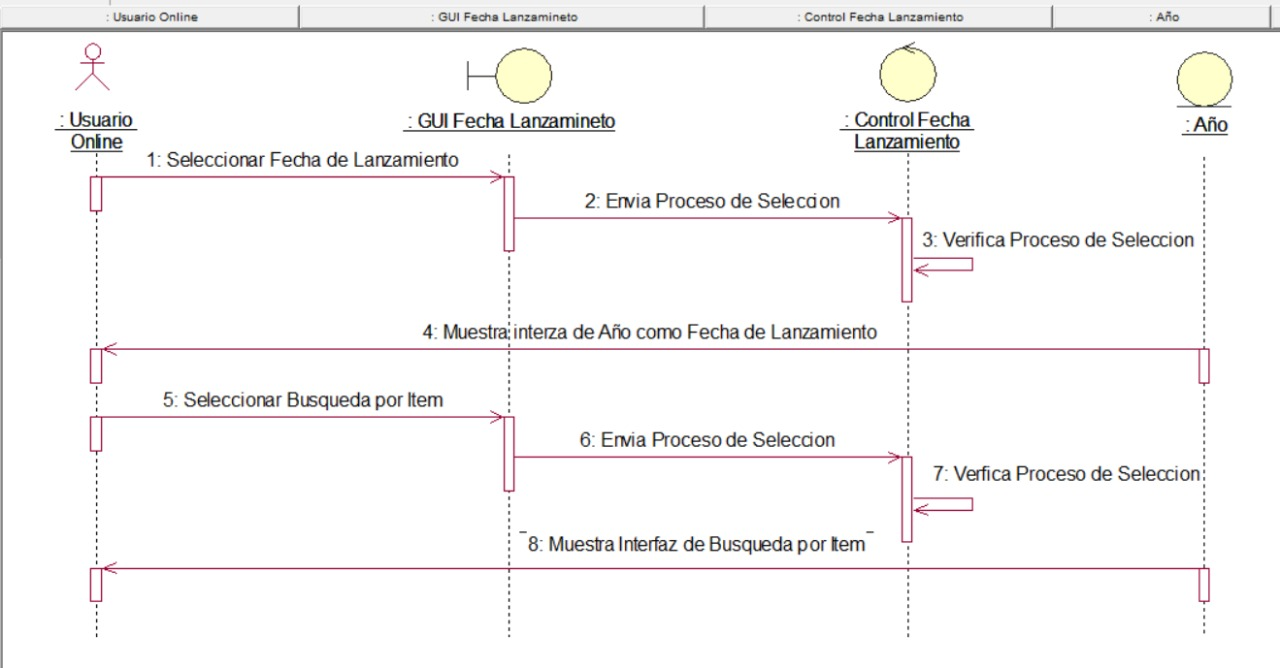
\includegraphics[width=14cm]{./Imagenes/Secuencia4}
\end{center}
\thinspace
\thinspace
\thinspace
\thinspace
\thinspace
\thinspace
\thinspace
\thinspace
\thinspace
\thinspace
\thinspace
\thinspace
\thinspace
\thinspace
Seleccionar Documento
\thinspace
\thinspace
\thinspace
\thinspace
\thinspace
\thinspace
\thinspace
\thinspace
\thinspace
\thinspace
\thinspace
\thinspace
\begin{center}
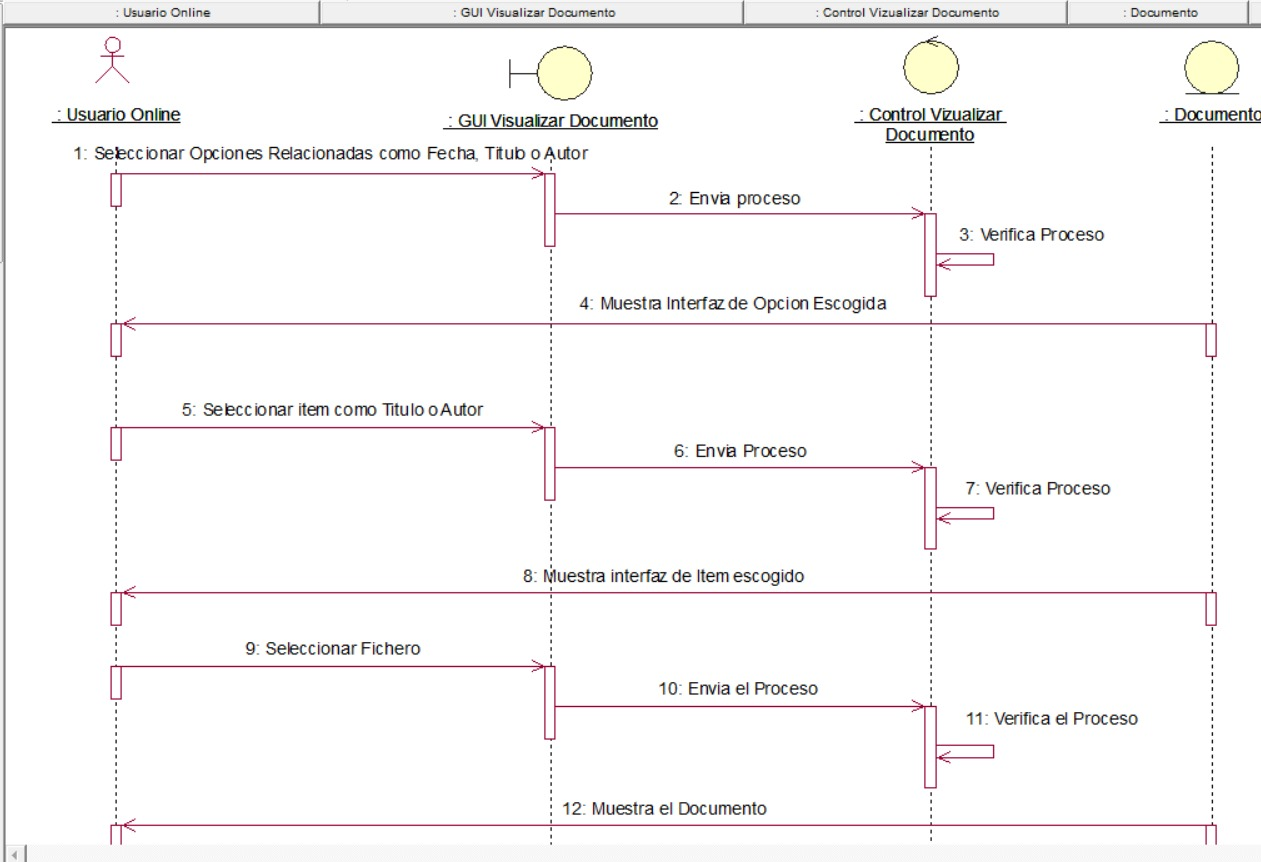
\includegraphics[width=14cm]{./Imagenes/Secuencia5}
\end{center}
\subsection{DISEÑO (DIAGRAMA DE CLASES, MODELO ENTIDAD RELACION)}
\subsubsection{DIAGRAMA DE CLASES}
\subsubsection{MODELO ENTIDAD RELACION}


\begin{center}
\includegraphics[width=20cm]{./Imagenes/Entidad}
\end{center}

\subsection{DISEÑO INTERFAZ DE USUARIO (PANTALLAS Y METODOS DE CLASES UTILIZADOS)}
\subsubsection{INTERFACES}
\subsubsection{METODOS DE CLASES UTILIZADOS}
\end{document}
